\section{Diskrétní obraz, jeho vlastnosti a reprezentace (model kamery, projekce, digitalizace, metriky), binární, šedotónový a barevný obraz - barevné formáty, souborové formáty.}

\subsection*{Model kamery a projekce}
Obraz vzniká projekcí 3D scény na 2D snímací rovinu. Nejjednodušší model je dírková kamera (pinhole).
Používá perspektivní projekci, proto se vzdálenější objekty zobrazují menší.
\begin{itemize}
    \item \textbf{Perspektivní projekce} převádí bod \(P=[X,Y,Z]\) na souřadnice obrazu:
          \begin{equation}
              x = f\frac{X}{Z}, \qquad y = f\frac{Y}{Z}
          \end{equation}
          kde \(f\) je ohnisková vzdálenost
    \item \textbf{Ortografická projekce} zanedbá změnu měřítka s hloubkou. Hodí se, pokud jsou změny \(Z\) malé vůči vzdálenosti kamery
    \item Reálný snímací řetězec navíc ovlivňuje osvětlení, optika, clona, expozice, senzor a A/D převod
\end{itemize}

\begin{figure}[h!]
    \centering
    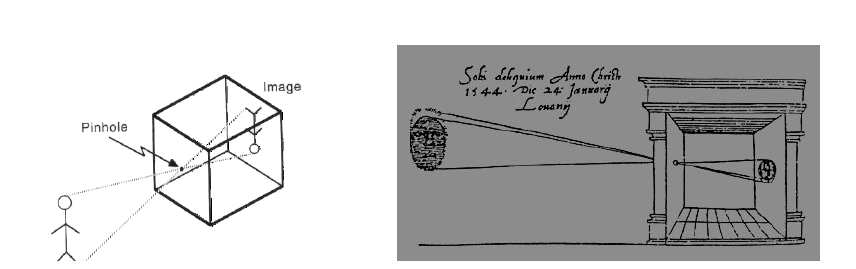
\includegraphics[width=0.9\textwidth]{img/camera_model.png}
\end{figure}

\subsection*{Obrazová funkce}
Spojitý šedotónový obraz lze popsat obrazovou funkcí:
\begin{equation}
    g_c: \Omega_c \subset \mathbb{R}^2 \rightarrow \mathbb{R}
\end{equation}
Po digitalizaci vzniká diskrétní obraz:
\begin{equation}
    g_d: \Omega_d \subset \mathbb{Z}^2 \rightarrow \mathbb{Z}
\end{equation}
Prakticky jde o matici pixelů \(M \times N\), kde každý pixel má jasovou nebo barevnou hodnotu.

\subsection*{Digitalizace}
Digitalizace má dvě části:
\begin{itemize}
    \item \textbf{Vzorkování} - převod spojitých souřadnic na pravidelnou mřížku pixelů. Určuje prostorové rozlišení
    \item \textbf{Kvantování} - převod spojité hodnoty jasu na konečný počet úrovní
\end{itemize}
Při kvantování do \(b\) bitů je počet jasových úrovní:
\begin{equation}
    K = 2^b
\end{equation}
Časté hodnoty jsou 1 bit pro binární obraz, 8 bitů pro šedotónový obraz a 24 bitů pro RGB obraz.
Při nízkém rozlišení vzniká ztráta detailů, při malém počtu úrovní vznikají kvantizační artefakty.
Vzorkovací frekvence musí respektovat prostorový Nyquistův princip, jinak vzniká aliasing.

\begin{figure}[h!]
    \centering
    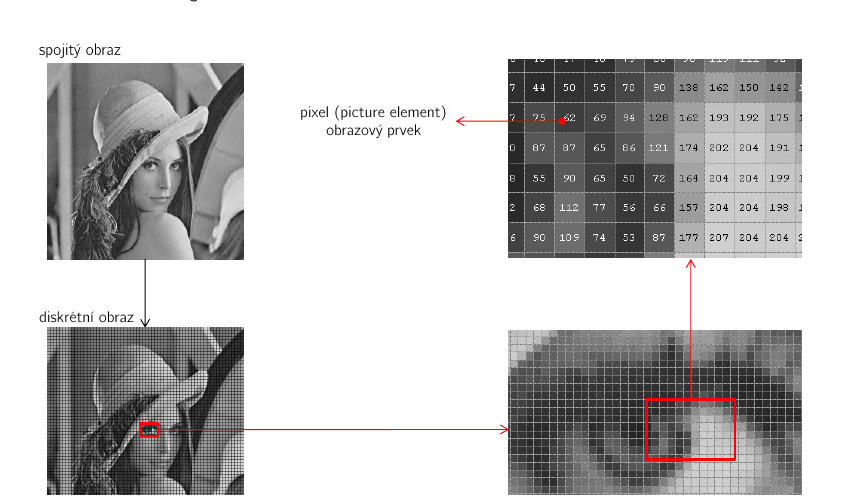
\includegraphics[width=0.85\textwidth]{img/digitalizace.png}
\end{figure}

\subsection*{Vlastnosti diskrétního obrazu}
\begin{itemize}
    \item \textbf{Rozlišení} - počet pixelů, např. \(1920 \times 1080\)
    \item \textbf{Bitová hloubka} - počet bitů na pixel nebo na kanál
    \item \textbf{Dynamický rozsah} - interval možných hodnot jasu
    \item \textbf{Šum a zkreslení} - nežádoucí složky vzniklé při snímání, přenosu nebo digitalizaci
    \item \textbf{Paměťová náročnost} - přibližně \(M \cdot N \cdot b\) bitů pro jeden kanál
\end{itemize}

\subsection*{Okolí bodu a metriky}
V diskrétním obrazu se často pracuje s okolím pixelu:
\begin{itemize}
    \item \textbf{4-okolí} - levý, pravý, horní a dolní soused
    \item \textbf{8-okolí} - 4-okolí doplněné o diagonální sousedy
    \item \textbf{6-okolí} - používá se u hexagonální mřížky
\end{itemize}
Vzdálenost bodů lze měřit různými metrikami:
\begin{itemize}
    \item městská metrika: \(d_1(R,S)=\sum_i |r_i-s_i|\)
    \item eukleidovská metrika: \(d_2(R,S)=\sqrt{\sum_i (r_i-s_i)^2}\)
    \item šachovnicová metrika: \(d_\infty(R,S)=\max_i |r_i-s_i|\)
\end{itemize}

\begin{figure}[h!]
    \centering
    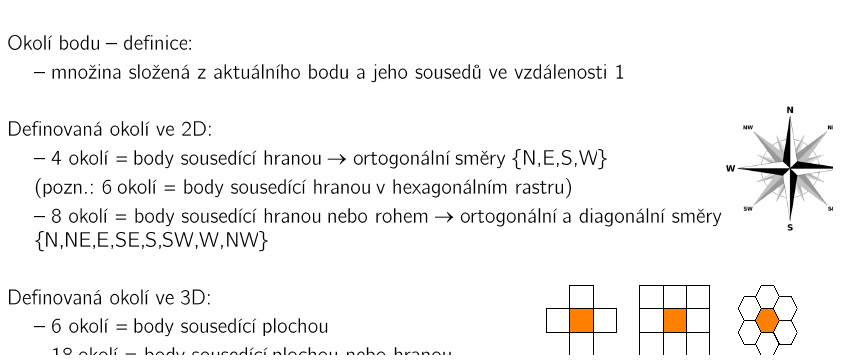
\includegraphics[width=0.75\textwidth]{img/metriky_okoli.png}
\end{figure}

\subsection*{Binární, šedotónový a barevný obraz}
\begin{itemize}
    \item \textbf{Binární obraz} - hodnoty pouze 0/1, vhodný pro masky, segmentaci a morfologii
    \item \textbf{Šedotónový obraz} - jedna jasová složka, typicky \(0\) až \(255\)
    \item \textbf{Barevný obraz} - několik složek, nejčastěji RGB:
          \begin{equation}
              f(x,y)=\left[f_R(x,y), f_G(x,y), f_B(x,y)\right]
          \end{equation}
\end{itemize}

\subsection*{Barevné modely}
\begin{itemize}
    \item \textbf{RGB, RGBA} - aditivní model, používá se u displejů a kamer. Alfa kanál udává průhlednost
    \item \textbf{CMY, CMYK} - substraktivní model pro tisk. Složka K je černá barva
    \item \textbf{HSV, HLS} - intuitivní modely: odstín, sytost, jas/světlost
    \item \textbf{YUV, YCbCr} - oddělení jasové složky od chrominančních složek, používá se u videa, JPEG a MPEG
    \item \textbf{CIE XYZ} - standardizovaný model pro popis barev a barevných rozsahů zařízení
\end{itemize}
U běžných jednosnímačových kamer se místo tří separátních čipů používá barevná mozaika CFA (Color Filter Array).
Každý pixel snímá jen jednu barevnou složku, ostatní se dopočítají z okolí -- tento proces se nazývá demosaicing.
Nejběžnější vzory CFA:
\begin{itemize}
    \item RGB Bayer -- nejpoužívanější, 50\,\% zelených, 25\,\% červených, 25\,\% modrých pixelů
    \item CYGM, CYYM -- alternativní vzory pro vyšší citlivost (Kodak)
    \item RGBE, RGBW (Sony/Kodak) -- modifikace Bayeru s bílým nebo smaragdovým pixelem pro lepší expozici
\end{itemize}

\begin{figure}[h!]
    \centering
    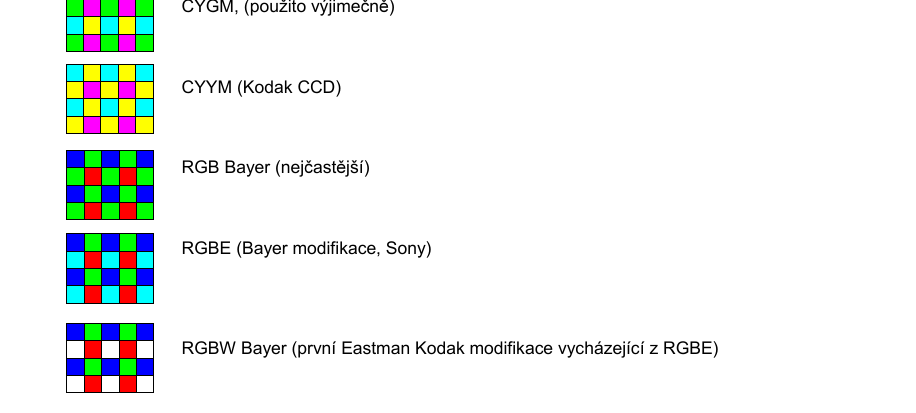
\includegraphics[width=0.85\textwidth]{img/bayer_mozaika.png}
\end{figure}

\subsection*{Souborové formáty}
Obrazové formáty se dělí hlavně podle reprezentace a komprese:
\begin{itemize}
    \item \textbf{RAW/BMP} - jednoduché rastrové uložení, bez komprese nebo s minimální kompresí
    \item \textbf{PCX} - starší formát, často RLE komprese
    \item \textbf{GIF} - LZW komprese, paleta do 256 barev, animace a průhlednost
    \item \textbf{PNG} - bezeztrátová komprese LZ77/Deflate, alfa kanál, vhodné pro grafiku a text
    \item \textbf{JPEG} - ztrátová komprese přes YCbCr, podvzorkování barev, DCT, kvantování a entropické kódování
    \item \textbf{TIFF} - univerzální formát pro profesionální práci, mnoho variant a kompresí
    \item \textbf{SVG} - vektorový formát, ukládá grafická primitiva místo pixelů
\end{itemize}

\begin{figure}[h!]
    \centering
    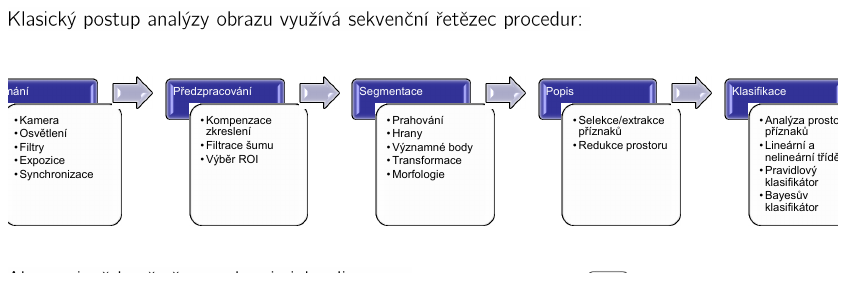
\includegraphics[width=0.9\textwidth]{img/retezec_zpracovani.png}
\end{figure}

\newpage

\section{Konvoluční integrál, korelace obrazových signálů, okolí bodu, lineární a nelineární filtry (masky - detekce hran a rohů, filtrace šumu), typy šumu.}

\subsection*{2D systém, PSF a konvoluce}
Obrazové zpracování lze chápat jako 2D systém, který ze vstupního obrazu \(f(x,y)\) vytvoří výstupní obraz \(g(x,y)\).
Odezva systému na bodový impuls se nazývá rozptylová funkce PSF (point spread function).

Pro izoplanární lineární systém, jehož PSF nezávisí na poloze v obraze, platí konvoluční integrál:
\begin{equation}
    g(x,y)=\int_{-\infty}^{\infty}\int_{-\infty}^{\infty}
    f(\xi,\eta)h(x-\xi,y-\eta)d\xi d\eta
\end{equation}
V diskrétním obrazu se používá konvoluce s maskou:
\begin{equation}
    g(k,l)=\sum_{i=-M/2}^{M/2}\sum_{j=-N/2}^{N/2}
    f(k-i,\,l-j)\,h(i,j)
\end{equation}
Maska \(h\) je lokální PSF, tedy konvoluční jádro. Pro symetrická jádra (Gaussovo, průměrovací) je konvoluce totožná s křížovou korelací.

\begin{figure}[h!]
    \centering
    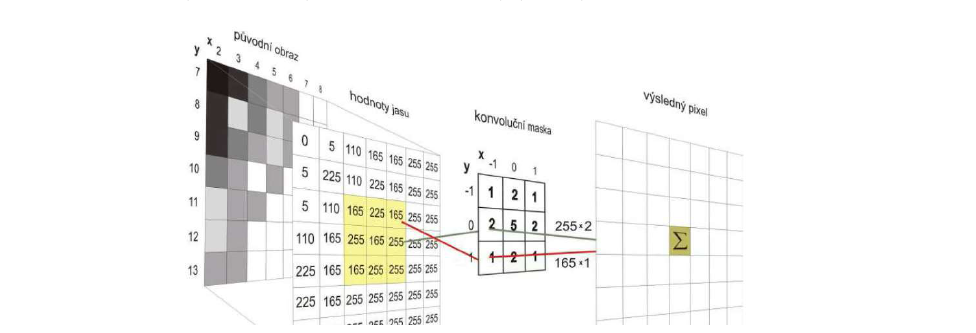
\includegraphics[width=0.82\textwidth]{img/konvoluce_maska.png}
\end{figure}

\subsection*{Korelace}
Korelace měří podobnost dvou obrazových signálů při různém posunu. Používá se pro hledání vzoru v obrazu.
\begin{equation}
    r_{fg}(m,n)=\sum_x\sum_y f(x,y)g(x+m,y+n)
\end{equation}
\begin{itemize}
    \item \textbf{Křížová korelace} - podobnost dvou různých obrazů nebo obrazu a šablony
    \item \textbf{Autokorelace} - korelace obrazu se sebou samým, hledání periodicity a opakujících se struktur
    \item Ve frekvenční oblasti lze korelaci počítat rychleji přes Fourierovu transformaci
\end{itemize}

\subsection*{Lineární filtry}
Lineární filtr je dán konvolucí obrazu s maskou. Platí superpozice, komutativita a asociativita.
\begin{itemize}
    \item \textbf{Průměrovací filtr} - potlačuje náhodný šum, ale rozmazává hrany
    \item \textbf{Vážený průměr} - střed masky má větší váhu, např. aproximace Gaussova filtru
    \item \textbf{Gaussův filtr} - hladké vyhlazení, často používaný před detekcí hran
    \item \textbf{Derivační filtry} - zvýrazňují změny jasu, tedy hrany
    \item \textbf{Ostřící filtry} - přičítají vysokofrekvenční složku k původnímu obrazu
\end{itemize}
U vyhlazovacích filtrů má být součet koeficientů masky roven 1, aby se neměnil celkový jas obrazu.
U hranových masek bývá součet koeficientů 0, aby se potlačila stejnosměrná složka.

\subsection*{Nelineární filtry}
Nelineární filtr nelze popsat prostou konvolucí.
\begin{itemize}
    \item \textbf{Mediánový filtr} - nahradí pixel mediánem okolí, velmi dobrý pro impulsní šum typu sůl a pepř
    \item \textbf{Min/max filtr} - zvýrazňuje tmavé nebo světlé lokální struktury
    \item \textbf{Modus} - nahrazení nejčastější hodnotou v okolí
    \item \textbf{Morfologické filtry} - pracují se strukturním elementem, vhodné hlavně pro binární obrazy
\end{itemize}

\subsection*{Typy šumu}
\begin{itemize}
    \item \textbf{Impulsní šum} - sůl a pepř, náhodné bílé a černé body
    \item \textbf{Gaussovský šum} - náhodný šum s normálním rozdělením
    \item \textbf{Poissonovský šum} - vzniká při počítání fotonů, typický pro snímače při slabém osvětlení
    \item \textbf{Bílý šum} - má rovnoměrné zastoupení frekvencí
    \item \textbf{Kvantizační šum} - důsledek nedostatečného počtu jasových úrovní
    \item \textbf{Aditivní šum} - k obrazu se přičítá, typicky při snímání nebo přenosu
    \item \textbf{Multiplikativní šum} - násobí obraz, např. nerovnoměrnost osvětlení nebo raster
\end{itemize}

\begin{figure}[h!]
    \centering
    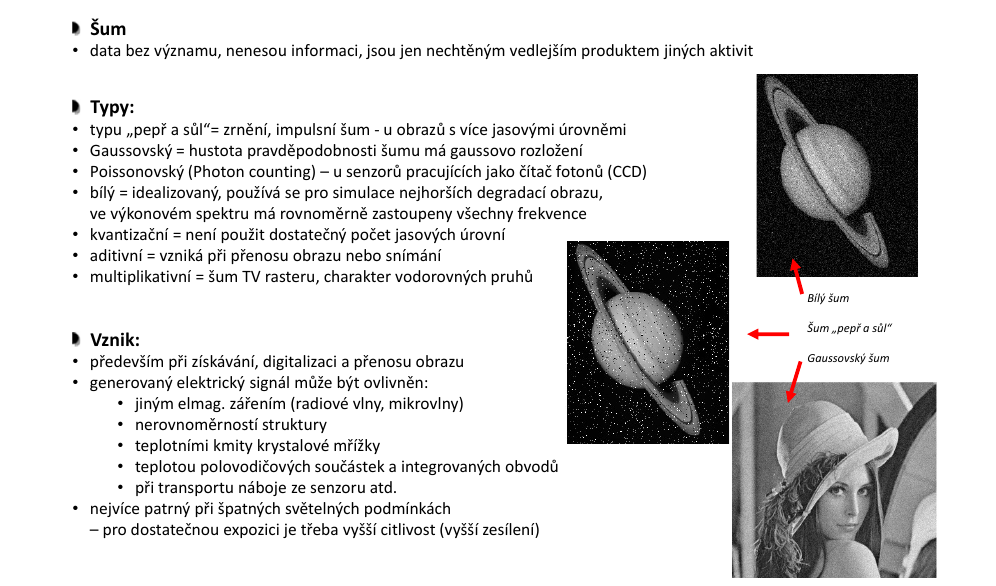
\includegraphics[width=0.9\textwidth]{img/typy_sumu.png}
\end{figure}

\subsection*{Detekce hran}
Hrana je místo s výraznou změnou jasu. Detekuje se pomocí derivací obrazové funkce.
Gradient:
\begin{equation}
    \nabla f(x,y)=
    \begin{bmatrix}
        G_x\\G_y
    \end{bmatrix}
    =
    \begin{bmatrix}
        \frac{\partial f}{\partial x}\\
        \frac{\partial f}{\partial y}
    \end{bmatrix}
\end{equation}
Velikost gradientu:
\begin{equation}
    |\nabla f|=\sqrt{G_x^2+G_y^2} \approx |G_x|+|G_y|
\end{equation}
Směr hrany (orientace normály):
\begin{equation}
    \theta = \mathrm{atan2}(G_y,\,G_x)
\end{equation}

Časté hranové masky:
\begin{itemize}
    \item \textbf{Robertsův operátor} - malé \(2\times2\) masky, citlivý na šum
    \item \textbf{Prewittův operátor} - první derivace v \(3\times3\) okolí
    \item \textbf{Sobelův operátor} - podobný Prewittové, ale větší váha středu:
          \[
              S_x=
              \begin{bmatrix}
                  -1&0&1\\
                  -2&0&2\\
                  -1&0&1
              \end{bmatrix},
              \quad
              S_y=
              \begin{bmatrix}
                  -1&-2&-1\\
                  0&0&0\\
                  1&2&1
              \end{bmatrix}
          \]
    \item \textbf{Laplacián} - druhá derivace, hledá průchod nulou:
          \[
              L=
              \begin{bmatrix}
                  0&1&0\\
                  1&-4&1\\
                  0&1&0
              \end{bmatrix}
          \]
    \item \textbf{LoG} - Laplacian of Gaussian, nejprve vyhladí šum a poté hledá hrany
    \item \textbf{Cannyho detektor} - vyhlazení, gradient, potlačení nemaxim, hysterezní prahování
\end{itemize}

\subsection*{Detekce rohů}
Roh je bod, kde se jas výrazně mění ve více směrech.
\begin{itemize}
    \item \textbf{Moravcův operátor} - sleduje změnu intenzity při posunu okna různými směry
    \item \textbf{Harrisův detektor} - vychází z matice gradientů v okolí bodu
    \item Hrana má velkou změnu v jednom směru, roh ve dvou na sebe nezávislých směrech
\end{itemize}

\newpage

\section{Jasové transformace (histogram, kumulovaný histogram - ekvalizace, jasové korekce), geometrické transformace
(aproximace, bilineární a afinní transformace, homogenní souřadnice, interpolace souřadnic, korekce zkreslení, rotace /
měřítko).}

\subsection*{Jasové transformace}
Jasová transformace mění hodnoty pixelů podle pravidla \(T\), ale nemění geometrii obrazu.
Vstupem i výstupem je obraz stejného rozlišení a stejné souřadnicové mřížky.

Rozdělení:
\begin{itemize}
    \item \textbf{Globální} - nový jas pixelu se počítá z celého obrazu, např. ekvalizace histogramu
    \item \textbf{Lokální} - nový jas se počítá z okolí pixelu, např. vyhlazení, medián, lokální kontrast
    \item \textbf{Bodové} - nový jas závisí jen na původní hodnotě daného pixelu
\end{itemize}

\subsection*{Histogram}
Histogram udává četnost jednotlivých jasových úrovní:
\begin{equation}
    h(q)=\#\{(x,y): f(x,y)=q\}
\end{equation}
Relativní histogram lze chápat jako odhad pravděpodobnosti výskytu jasu \(q\).
Používá se pro posouzení kontrastu a jako základ pro ekvalizaci.

\subsection*{Kumulovaný histogram a ekvalizace}
Kumulovaný histogram:
\begin{equation}
    h_k(q)=\sum_{i=0}^{q}h(i)
\end{equation}
Normalizovaný kumulovaný histogram se používá jako převodní charakteristika ekvalizace:
\begin{equation}
    q' = (K-1)\frac{h_k(q)}{M\cdot N}
\end{equation}
Cílem ekvalizace je roztáhnout využitý rozsah jasů a zvýšit kontrast.
Nevýhodou může být zvýraznění šumu nebo nepřirozený vzhled obrazu.

\begin{figure}[h!]
    \centering
    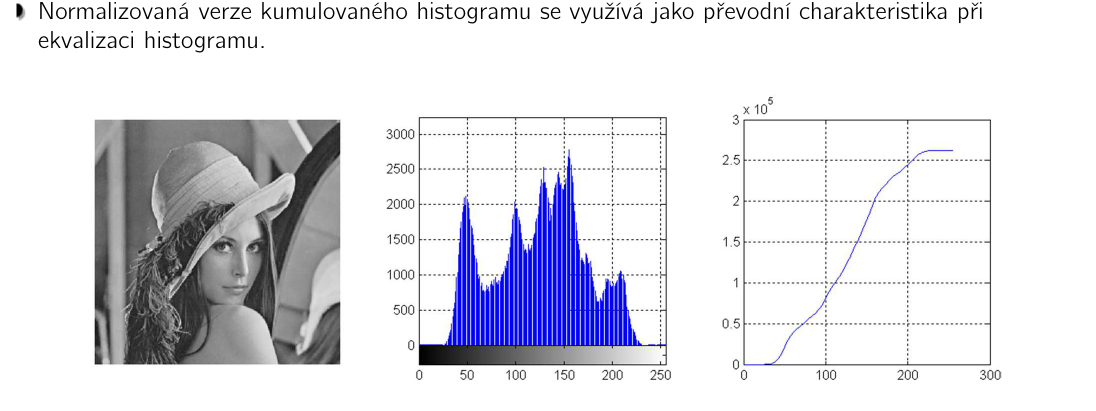
\includegraphics[width=0.88\textwidth]{img/histogram_kumulovany.png}
\end{figure}

\subsection*{Bodové jasové transformace}
Typické bodové transformace:
\begin{itemize}
    \item negativ: \(g=K-1-f\)
    \item lineární změna kontrastu: \(g=a f+b\)
    \item prahování: \(g=1\) pro \(f \ge T\), jinak \(g=0\)
    \item gamma korekce: \(g=c f^\gamma\)
    \item saturace a ořez rozsahu na interval \(\langle0;K-1\rangle\)
\end{itemize}

\subsection*{Jasové korekce}
Jasová korekce kompenzuje systematickou chybu při pořízení obrazu:
\begin{itemize}
    \item nerovnoměrné osvětlení,
    \item rozdílná citlivost prvků snímače,
    \item vadné pixely,
    \item nedokonalá přenosová funkce optické soustavy
\end{itemize}
Často se předpokládá multiplikativní degradace:
\begin{equation}
    f(x,y)=e(x,y)g(x,y)
\end{equation}
kde \(g\) je nekorigovaný obraz, \(e\) degradační funkce a \(f\) korigovaný obraz.
Degradační funkce se určí analyticky nebo z etalonového snímku.

\subsection*{Geometrické transformace}
Geometrická transformace mění souřadnice pixelů:
\begin{equation}
    (x',y') = T(x,y)
\end{equation}
Má dvě části:
\begin{itemize}
    \item transformace souřadnic,
    \item interpolace jasové hodnoty v nové poloze
\end{itemize}
Problém diskrétního obrazu je, že transformované souřadnice jsou obecně neceločíselné. Proto se musí interpolovat.
Při přímém mapování mohou vznikat díry nebo překryvy, v praxi se často používá zpětné mapování z výstupní mřížky do vstupního obrazu.

\subsection*{Aproximace transformace}
Obecná transformace se často nahrazuje polynomiální aproximací:
\begin{equation}
    x'=\sum_{r=0}^{n}\sum_{k=0}^{n-r}a_{rk}x^r y^k,\qquad
    y'=\sum_{r=0}^{n}\sum_{k=0}^{n-r}b_{rk}x^r y^k
\end{equation}
Koeficienty se určují z odpovídajících si bodů, typicky metodou nejmenších čtverců.
Pro mírné zkreslení stačí nízký stupeň polynomu.

\subsection*{Afinní a bilineární transformace}
Afinní transformace:
\begin{equation}
    x'=a_0+a_1x+a_2y,\qquad y'=b_0+b_1x+b_2y
\end{equation}
Umí popsat posun, rotaci, měřítko a zkosení. Zachovává rovnoběžnost přímek.

Bilineární transformace přidává člen \(xy\) do každé souřadnicové složky:
\begin{equation}
    x'=a_0+a_1x+a_2y+a_3xy,\qquad y'=b_0+b_1x+b_2y+b_3xy
\end{equation}
Používá se pro modelování jednoduchých nelineárních zkreslení (např. perspektiva malého pole pohledu).

\subsection*{Homogenní souřadnice}
Homogenní souřadnice přidávají jednu dimenzi navíc. Bod \([x,y]^T\) se zapíše jako \([x,y,1]^T\).
Afinní transformace pak má maticový tvar:
\begin{equation}
    \begin{bmatrix}
        x'\\y'\\1
    \end{bmatrix}
    =
    \begin{bmatrix}
        a_1&a_2&a_0\\
        b_1&b_2&b_0\\
        0&0&1
    \end{bmatrix}
    \begin{bmatrix}
        x\\y\\1
    \end{bmatrix}
\end{equation}
Výhodou je snadné skládání transformací násobením matic.

\subsection*{Interpolace}
Interpolace odhaduje jas v neceločíselné souřadnici.
\begin{itemize}
    \item \textbf{Nejbližší soused} - nejrychlejší, ale vytváří schodovitý vzhled
    \item \textbf{Bilineární interpolace} - používá \(2\times2\) okolí, plynulejší výsledek
    \item \textbf{Bikubická interpolace} - používá \(4\times4\) okolí, lepší kvalita, vyšší výpočetní náročnost
    \item \textbf{Spline/sinc} - kvalitnější aproximace, vhodné pro přesnější převzorkování
\end{itemize}

\begin{figure}[h!]
    \centering
    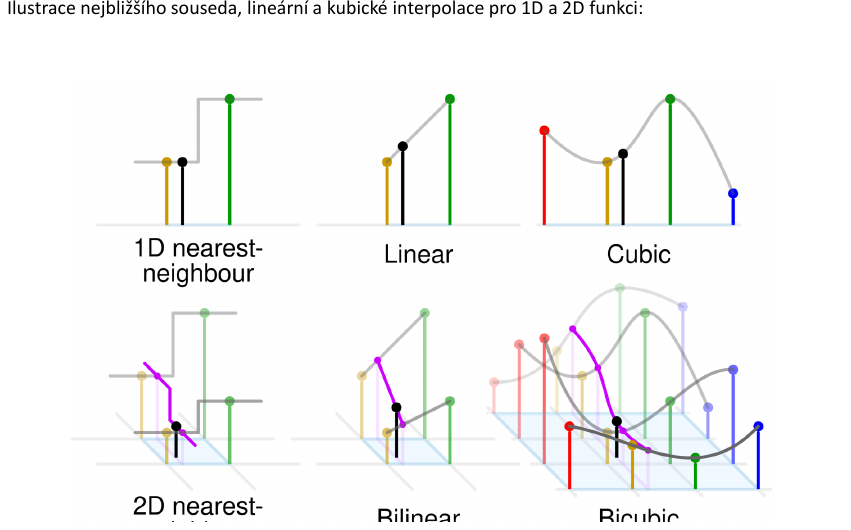
\includegraphics[width=0.78\textwidth]{img/interpolace_metody.png}
\end{figure}

\subsection*{Korekce zkreslení}
Korekce zkreslení hledá transformaci, která převádí zkreslený obraz na pravidelnou mřížku.
\begin{itemize}
    \item \textbf{Radiální zkreslení} - soudek nebo poduška, závisí na vzdálenosti od středu obrazu
    \item \textbf{Tangenciální zkreslení} - vzniká např. natočením optické osy vůči senzoru
    \item Transformace se určuje kalibrací pomocí známé kalibrační mřížky
\end{itemize}
Radiální model (soudek / poduška):
\begin{equation}
    x'=x(1+\kappa_1 r^2+\kappa_2 r^4+\kappa_3 r^6), \qquad
    y'=y(1+\kappa_1 r^2+\kappa_2 r^4+\kappa_3 r^6)
\end{equation}
kde \(r^2=x^2+y^2\) je kvadrát vzdálenosti od středu obrazu a \(\kappa_i\) jsou koeficienty radiálního zkreslení.

Tangenciální model (naklopení optické osy vůči senzoru):
\begin{equation}
    x'=x+2\rho_1 y+\rho_2(r^2+2x^2), \qquad
    y'=y+2\rho_2 x+\rho_1(r^2+2y^2)
\end{equation}
kde \(\rho_1, \rho_2\) jsou koeficienty tangenciálního zkreslení.

\begin{figure}[h!]
    \centering
    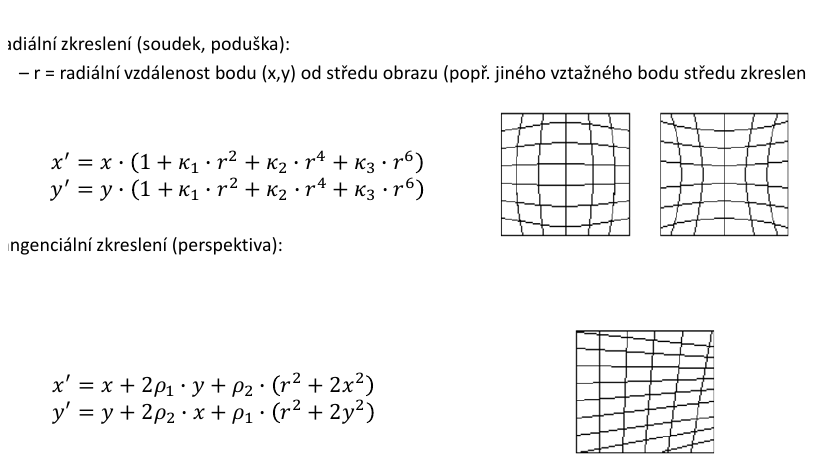
\includegraphics[width=0.78\textwidth]{img/geometricke_zkresleni.png}
\end{figure}

\subsection*{Rotace a měřítko}
Rotace o úhel \(\alpha\):
\begin{equation}
    \begin{bmatrix}
        x'\\y'\\1
    \end{bmatrix}
    =
    \begin{bmatrix}
        \cos\alpha&-\sin\alpha&0\\
        \sin\alpha&\cos\alpha&0\\
        0&0&1
    \end{bmatrix}
    \begin{bmatrix}
        x\\y\\1
    \end{bmatrix}
\end{equation}
Změna měřítka:
\begin{equation}
    x'=m_x x,\qquad y'=m_y y
\end{equation}
Při zvětšení i zmenšení obrazu je nutná interpolace. Při zmenšení je vhodné předem potlačit vysoké frekvence, aby nevznikl aliasing.

\newpage

\section{Morfologické operace a integrální transformace (využití FT pro zpracování vícerozměrných signálů - vzorce,
vlastnosti, výhody a nevýhody, typy a tvorba filtrů, korelace a autokorelace).}

\subsection*{Matematická morfologie}
Matematická morfologie zpracovává obraz přes tvar objektů. Původně byla určena pro binární obrazy,
později se rozšířila i na šedotónové obrazy.

Binární obraz lze chápat jako množinu bodů \(I \subset \mathbb{Z}^2\).
Morfologická operace pracuje s obrazem \(I\) a strukturním elementem \(B\), který určuje tvar a velikost lokálního okolí.

\subsection*{Dilatace}
Dilatace zvětšuje objekty a zaplňuje malé mezery:
\begin{equation}
    I\oplus B=\{p\in E^2: p=i+b,\; i\in I,\; b\in B\}
\end{equation}
Použití:
\begin{itemize}
    \item zvětšení objektů,
    \item spojení blízkých oblastí,
    \item zaplnění malých děr
\end{itemize}

\subsection*{Eroze}
Eroze zmenšuje objekty a odstraňuje tenké výběžky:
\begin{equation}
    I\ominus B=\{p\in E^2: p+b\in I,\; \forall b\in B\}
\end{equation}
Použití:
\begin{itemize}
    \item odstranění drobného šumu,
    \item oddělení tenkých spojení,
    \item získání obrysu: \(O=I-(I\ominus B)\)
\end{itemize}

\subsection*{Otevření a uzavření}
Otevření je eroze následovaná dilatací:
\begin{equation}
    I\circ B=(I\ominus B)\oplus B
\end{equation}
Odstraňuje malé objekty a tenké spoje.

Uzavření je dilatace následovaná erozí:
\begin{equation}
    I\bullet B=(I\oplus B)\ominus B
\end{equation}
Spojuje blízké objekty a zaplňuje malé díry.

\begin{figure}[h!]
    \centering
    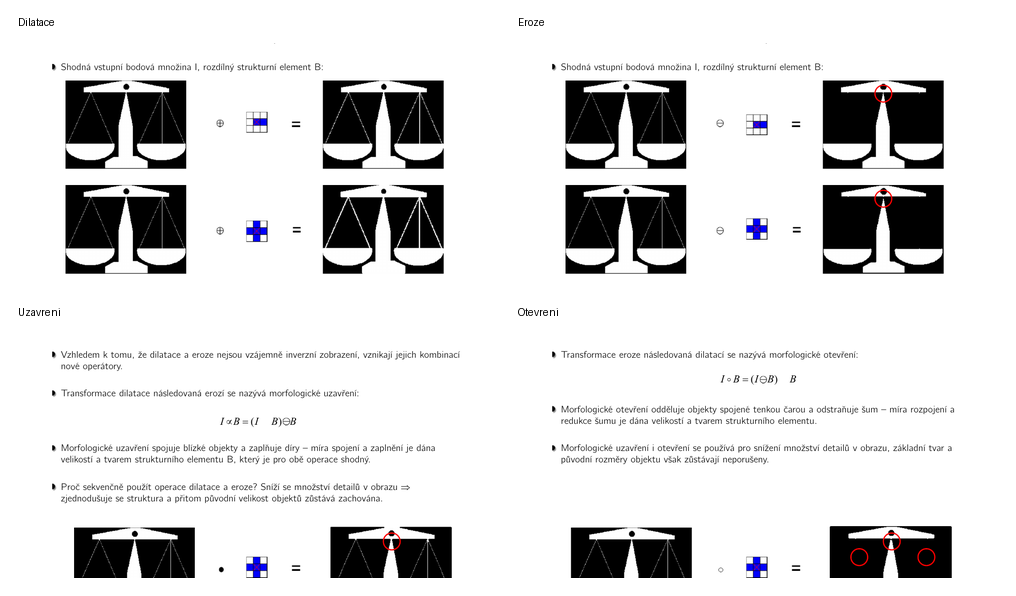
\includegraphics[width=0.9\textwidth]{img/morfologie_operace.png}
\end{figure}

\subsection*{Další morfologické operace}
\begin{itemize}
    \item \textbf{Skelet} - reprezentace objektu tenkou čarou zachovávající topologii
    \item \textbf{Tref či miň} - hledání přesné konfigurace objektu a pozadí pomocí dvojice sub-elementů
    \item \textbf{Ztenčování} - opakované odstraňování okrajových bodů, používá se pro aproximaci skeletu
    \item \textbf{Zesilování} - duální operace ke ztenčování
    \item \textbf{Golayova abeceda} - sada strukturních elementů pro ztenčování, zesilování a detekci tvarů
\end{itemize}

\begin{figure}[h!]
    \centering
    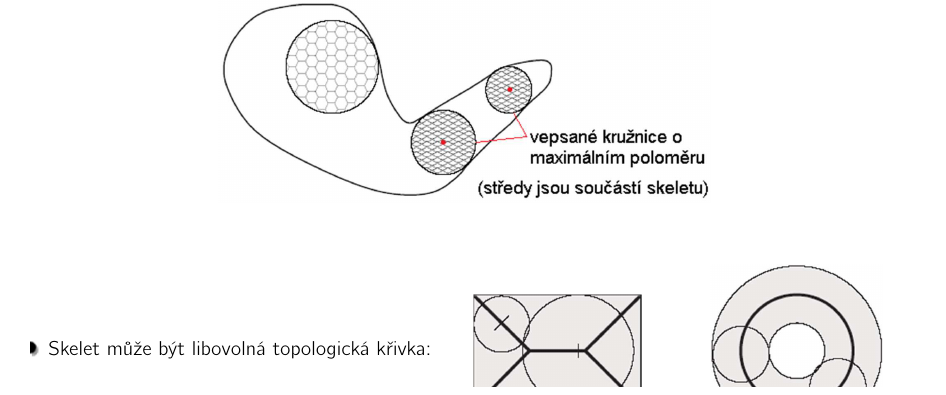
\includegraphics[width=0.82\textwidth]{img/skelet.png}
\end{figure}

\subsection*{Integrální transformace}
Integrální transformace převádí signál do jiné báze. Přímá a zpětná transformace umožňuje přechod mezi prostorovou a transformační doménou.
Obecně:
\begin{equation}
    F(u)=c\int f(x)\psi(x,u)dx
\end{equation}
\begin{equation}
    f(x)=C\int F(u)\psi^{-1}(x,u)du
\end{equation}
kde \(\psi\) je jádro transformace.

Typy:
\begin{itemize}
    \item Fourierova řada,
    \item Fourierova transformace,
    \item Laplaceova transformace,
    \item krátkodobá Fourierova transformace STFT,
    \item waveletová transformace,
    \item DCT používaná např. u JPEG
\end{itemize}

\subsection*{Fourierova transformace}
FT převádí signál z prostorové oblasti do oblasti prostorových frekvencí.
Nízké frekvence odpovídají pomalým změnám a plochám, vysoké frekvence hranám, detailům a šumu.

1D spojitá FT:
\begin{equation}
    F(\omega)=\int_{-\infty}^{\infty} f(t)e^{-j\omega t}dt
\end{equation}
Inverzní FT:
\begin{equation}
    f(t)=\frac{1}{2\pi}\int_{-\infty}^{\infty}F(\omega)e^{j\omega t}d\omega
\end{equation}

2D diskrétní FT:
\begin{equation}
    F(u,v)=\sum_{x=0}^{M-1}\sum_{y=0}^{N-1}
    f(x,y)e^{-j2\pi\left(\frac{ux}{M}+\frac{vy}{N}\right)}
\end{equation}
Inverzní 2D DFT:
\begin{equation}
    f(x,y)=\frac{1}{MN}\sum_{u=0}^{M-1}\sum_{v=0}^{N-1}
    F(u,v)e^{j2\pi\left(\frac{ux}{M}+\frac{vy}{N}\right)}
\end{equation}

\subsection*{Vlastnosti FT}
\begin{itemize}
    \item \textbf{Linearita} - transformace součtu je součet transformací
    \item \textbf{Bezeztrátovost} - přímá a zpětná FT vrátí původní signál, pokud se nemění koeficienty
    \item \textbf{Konvoluční věta} - konvoluce v prostoru je násobení ve frekvenční oblasti:
          \begin{equation}
              f*h \Longleftrightarrow F\cdot H
          \end{equation}
    \item \textbf{Separabilita} - 2D DFT lze počítat jako 1D DFT po řádcích a sloupcích
    \item \textbf{Periodicita} - DFT předpokládá periodické opakování signálu, okraje obrazu spolu sousedí
    \item \textbf{Symetrie} - pro reálný vstup je spektrum komplexně sdruženě symetrické
    \item \textbf{Amplituda a fáze} - amplituda říká zastoupení frekvence, fáze nese informaci o poloze struktur
\end{itemize}

\subsection*{Výhody a nevýhody FT}
Výhody:
\begin{itemize}
    \item rychlá realizace konvoluce přes FFT,
    \item vhodná pro velké filtry,
    \item snadná tvorba frekvenčních filtrů,
    \item detekce a potlačení periodického rušení,
    \item použití pro korelaci, autokorelaci, kompresi a rekonstrukci
\end{itemize}
Nevýhody:
\begin{itemize}
    \item globální transformace - špatná lokalizace změn v prostoru,
    \item pracuje jen s lineárními operacemi,
    \item spektrum je komplexní a paměťově náročnější,
    \item periodicita způsobuje artefakty na okrajích,
    \item ostré frekvenční filtry způsobují zvlnění v obraze
\end{itemize}

\subsection*{Frekvenční filtrace}
Ve frekvenční oblasti se obraz filtruje úpravou spektra:
\begin{equation}
    G(u,v)=F(u,v)H(u,v)
\end{equation}
Po inverzní transformaci vznikne filtrovaný obraz.

Typy filtrů:
\begin{itemize}
    \item \textbf{Dolní propust} - propustí nízké frekvence, vyhlazuje a potlačuje šum
    \item \textbf{Horní propust} - propustí vysoké frekvence, zvýrazňuje hrany
    \item \textbf{Pásmová propust/zádrž} - propustí nebo potlačí vybrané pásmo frekvencí
    \item \textbf{Směrový filtr} - reaguje na frekvence určité orientace
    \item \textbf{Notch filtr} - potlačuje izolované frekvenční složky, např. periodické rušení
\end{itemize}

\begin{figure}[h!]
    \centering
    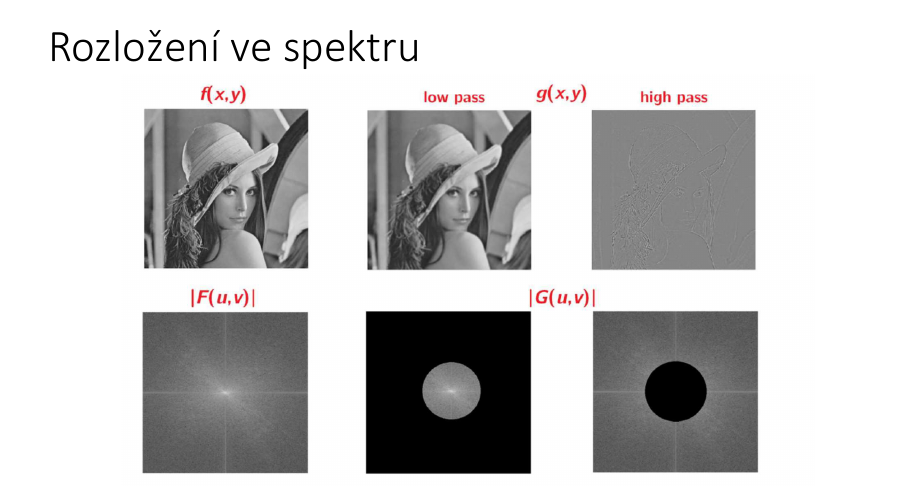
\includegraphics[width=0.82\textwidth]{img/ft_spektrum_filtry.png}
\end{figure}

\subsection*{Tvorba filtrů}
\begin{itemize}
    \item Filtr by neměl mít ostrou hranu, protože obdélníkový průběh ve frekvenci vytváří sinc průběh v prostoru
    \item Vhodné jsou hladké filtry: Gaussův, Butterworthův, Besselův, Čebyševův nebo oknové funkce
    \item Před filtrací je vhodné řešit okraje obrazu - nulové doplnění, opakování krajních hodnot, zrcadlení nebo oříznutí neplatných okrajů
    \item Při potlačení šumu se obvykle odstraňují vysoké frekvence, což současně rozmazává hrany
    \item Při ostření se zesilují vysoké frekvence, což současně může zvýraznit šum
\end{itemize}

\begin{figure}[h!]
    \centering
    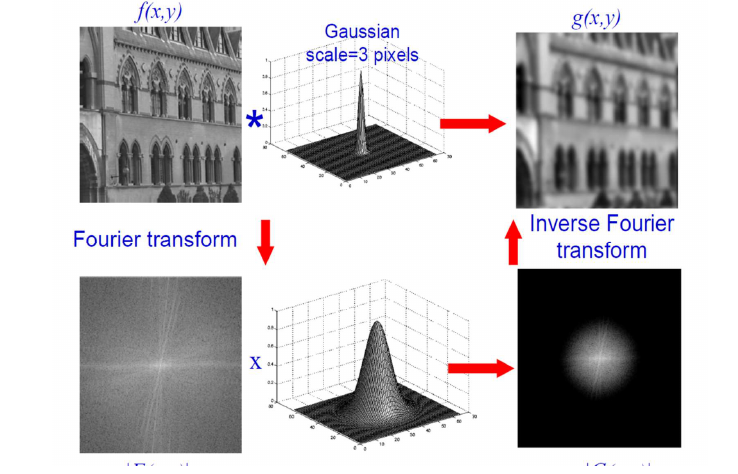
\includegraphics[width=0.82\textwidth]{img/ft_filtrace.png}
\end{figure}

\subsection*{Korelace a autokorelace přes FT}
Korelace lze počítat ve frekvenční oblasti násobením jednoho spektra komplexně sdruženým spektrem druhého signálu:
\begin{equation}
    r_{fg}=\mathcal{F}^{-1}\{F(u,v)\cdot G^*(u,v)\}
\end{equation}
Autokorelace:
\begin{equation}
    r_{ff}=\mathcal{F}^{-1}\{|F(u,v)|^2\}
\end{equation}
Použití:
\begin{itemize}
    \item hledání posunu mezi obrazy,
    \item detekce periodických struktur,
    \item porovnání obrazu se šablonou,
    \item registrace obrazů
\end{itemize}
